\documentclass[12pt]{article}


\usepackage[margin=1in]{geometry}


%load packages
\usepackage{epsfig}   %provides support for .eps
\usepackage{graphicx} %provides support for graphics
\usepackage{amsmath}  %some symbols / fonts


\usepackage{lipsum}

\title{An Example Document for ASTR288P}
\author{Sean Griffin}
\date{\today}

\begin{document}

\maketitle
\thispagestyle{empty} %gets rid of the page number on the first page
\newpage


\tableofcontents
\newpage

\section{Introduction}
\label{sec:intro}

Use this document as a reference for different environmnets. We will start with a citation \cite{exampleArticle} and another citation \cite{2017APh....91...34A}.

\section{Code Examples}
\label{sec:methods}

\subsection{Font Sizes}


\large I can make some text large. \Huge I can make some text huge! \tiny And other fonts really really small. \normalsize But often you just want normal size\footnote{Footnotes are also a thing.}\footnote{Even consecutive footnotes.}. 

We can add addtional text\footnote{\lipsum[3]} and continue about our day.

\subsection{Dummy Text}
The \texttt{lipsum} package allows me to generate dummy text:

\lipsum[4-5]

\section{Font Environments}


\begin{itemize}
\item \textbf{Bold}
\item \textit{Italic}
\item \textsc{Small caps}
\item \textsf{Sans serif font}
\item \textsl{Another font}
\item \texttt{Typewriter text}
\end{itemize}

Enumerated lists are a thing that exist, too: 

\begin{enumerate}

\item Item 1
\item Item 2
\item Another item
\item This item is long: \lipsum[1]

\end{enumerate}


\section{Equations}

\begin{equation}
\vec{F} = m\vec{a}
\end{equation}

\begin{align}
\vec{F} &= m\vec{a}\notag\\
 &= -G \frac{Mm}{r^2} \hat{r} \\
\mathbf{E} = \frac{q}{4\pi\epsilon_0} \left(\frac{\mathbf{r - r'}}{|\mathbf{r - r'}|^3}\right)
\end{align}

\begin{equation}
\label{eq:volume}
V = \frac{4}{3}\pi r^3 \propto r^3
\end{equation}

We can reference equations: Equation \ref{eq:volume}, sections: Section \ref{sec:intro}, and other environments.


\section*{An Unnumbered Section}

\begin{table}[t]
\centering
\begin{tabular}{cc|l|lr}
\hline\hline
5 & 5 & a & 12 & g\\
5 & 5 & a & 12 & g\\
word & another & another & another & another\\
a & b & c & d & e\\
\hline\hline
\end{tabular}

\caption{This is a table caption.}
\label{tab:exampleTable}
\end{table}

We can refer to the table: Table \ref{tab:exampleTable} and Figure \ref{fig:brittany}.

\begin{figure}[p]
\centering
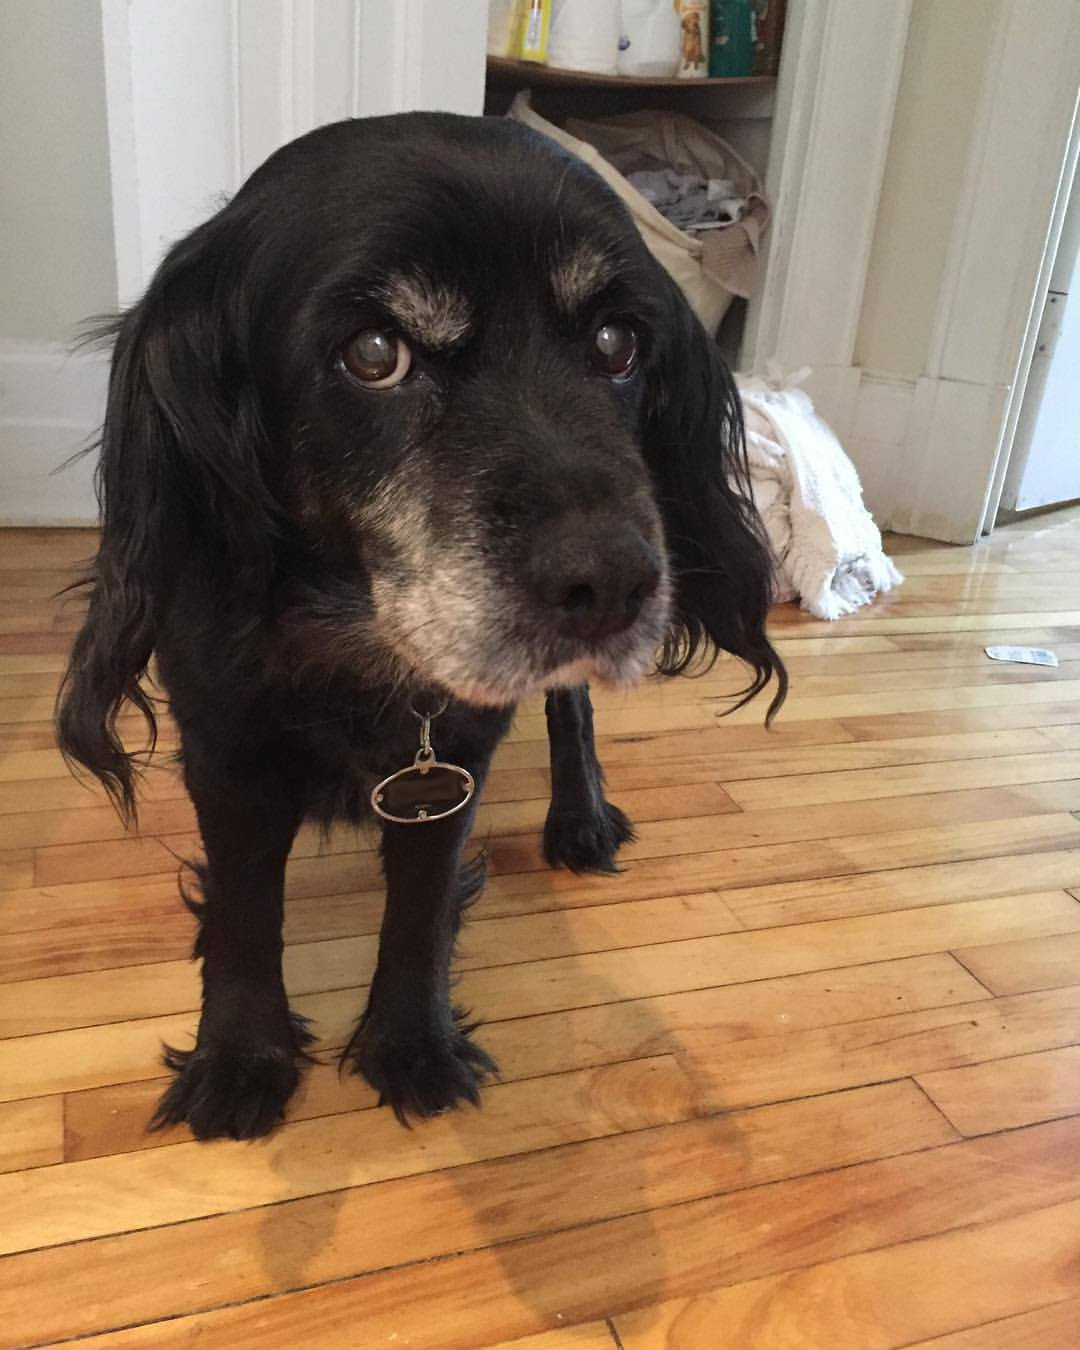
\includegraphics[width=0.6\textwidth]{figures/brittany}
\caption{This is Brittany. She's a good pupper.}
\label{fig:brittany}
\end{figure}

\section{Conclusions}


\subsection{}

\lipsum[1]

\subsubsection{}

\lipsum[5]

\subsubsection{}

\lipsum[1]

\subsection{}
\subsubsection{}
\lipsum[3]
\subsubsection{}
\lipsum[1]

%\bibliographystyle{unsrt}
%\bibliography{example_bib}

\bibliographystyle{apalike}
\bibliography{example_bib}

\end{document}
